\section{Methodology}
\label{sec:method}

% ---- Talking points written up as prose (your version: 05_methodology_draft.tex).

\subsection{Controller Design Pipeline}
\label{sec:pipeline}
The methods applied to the project correspond to the stages of the V-model in \cref{fig:vmodel}. It is a way for systems engineers to map out development across a product's life cycle \cite{seal_system_2018}. The first step in the design process is to determine the target use case and application of the product through background research, refining project objectives. To determine the system requirements for a controller the plant is modelled. The controller algorithms are then adpated to Simulink where a high-level structure forms. Based on this abstract model, components are selected for the controller PCB based on the requirements of the controller architecture. Selecting marketplace controllers and sensors, opens the door for firmware development because now there is a defined interface. The firmware's control code is then combined with the plant models in software-in-the-loop and QSPICE simulations, which give a theoretical approximation of the experiments. The system is tested in the electronics lab, and finally outdoors with a string of three PV modules, which is the core objective and ultimate validation of the system. \Cref{tab:phases} (\cref{app:timeline}) links each phase to its V-model counterpart and its primary artefact.

\begin{figure}[htbp]
  \centering
  % Controller design pipeline mapped onto the systems-engineering V-model.
% Drawn at print size (text width 17 cm): include without \resizebox.
\begin{tikzpicture}[x=1cm,y=1cm,font=\sffamily\scriptsize,
    ph/.style={draw,rounded corners=2pt,minimum width=32mm,minimum height=8.5mm,align=center,inner sep=2pt},
    arm/.style={-{Stealth[length=1.8mm]},thick,gray!70!black},
    ver/.style={{Stealth[length=1.6mm]}-{Stealth[length=1.6mm]},densely dashed,gray!70!black},
    vlab/.style={fill=white,inner sep=1pt,align=center,font=\sffamily\scriptsize\itshape,text=gray!40!black}]
  % the V itself: a band through the box centres
  \begin{scope}[on background layer]
    \draw[line width=12mm,gray!9,line cap=round,line join=round] (1.75,4.4) -- (6.15,0) -- (10.85,0) -- (15.25,4.4);
  \end{scope}
  % left arm: definition and decomposition (45 degrees)
  \node[ph,fill=blue!6]   (p0) at (1.75,4.4) {\textbf{0 Background research}\\\textit{Concept of operations}};
  \node[ph,fill=blue!6]   (p1) at (2.85,3.3) {\textbf{1 Analytical solution}\\\textit{System requirements}};
  \node[ph,fill=blue!6]   (p2) at (3.95,2.2) {\textbf{2 Model-in-the-loop}\\\textit{High-level design}};
  \node[ph,fill=blue!6]   (p3) at (5.05,1.1) {\textbf{3 Component selection}\\\textit{Detailed design}};
  % base of the V
  \node[ph,fill=yellow!15] (p4) at (6.85,0)  {\textbf{4 Firmware / software}\\\textit{Development}};
  \node[ph,fill=yellow!15] (p5) at (10.15,0) {\textbf{5 Software-in-the-loop}\\\textit{Unit verification}};
  % right arm: integration and verification
  \node[ph,fill=green!8]  (p6) at (11.95,1.1) {\textbf{6 QSPICE integration}\\\textit{Subsystem verification}};
  \node[ph,fill=green!8]  (p7) at (13.05,2.2) {\textbf{7 Bench test}\\\textit{System verification}};
  \node[ph,fill=green!8]  (p8) at (14.15,3.3) {\textbf{8 Solar test}\\\textit{System validation}};
  \node[ph,fill=green!8]  (p9) at (15.25,4.4) {\textbf{9 Synthesis}\\\textit{Acceptance}};
  % flow along the arms
  \foreach \a/\b in {p0/p1,p1/p2,p2/p3,p6/p7,p7/p8,p8/p9}{\draw[arm] (\a) -- (\b);}
  \draw[arm] (p3) -- (p4);
  \draw[arm] (p4) -- (p5);
  \draw[arm] (p5) -- (p6);
  % arm labels
  \node[rotate=-45,font=\sffamily\scriptsize\bfseries,text=blue!50!black] at (1.6,0.95) {definition and decomposition};
  \node[rotate=45,font=\sffamily\scriptsize\bfseries,text=green!35!black] at (15.4,0.95) {integration and verification};
  % verification pairs across the V
  \draw[ver] (p0) -- node[vlab]{report against the objectives} (p9);
  \draw[ver] (p1) -- node[vlab]{DC gain $G(N)$, $\tau$ vs $k$} (p8);
  \draw[ver] (p2) -- node[vlab]{validation suite, step metrics} (p7);
  \draw[ver] (p3) -- node[vlab]{sensing model,\\dead time, $R_{sw}$} (p6);
\end{tikzpicture}

  \caption[{Controller design pipeline mapped onto the systems-engineering V-model}]{Controller design pipeline mapped onto the systems-engineering V-model. Dashed links are the verification pairs used in \cref{sec:synthesis}.}
  \label{fig:vmodel}
\end{figure}
This method suits the problem because every phase produces a pass/fail artefact that the next phase consumes (model, then gains, then \code{params.h}, then the bench), so a fault is isolated at the level where it was introduced. The C control core is the same source file in software-in-the-loop, in QSPICE and in the firmware, so what is simulated is what is deployed.

The work was divided between control and power electronics. The hardware teammate, Son Nguyen, owned the power stage, the QSPICE schematic and the PCB layout. This project owned the control. The hand-over interface between the two was the QSPICE schematic and the sensor set. The team was proactive with regular progress updates occurring often more than twice a week. The supervisor, Assoc.\ Prof.\ Walker was updated eveyr fortnight either via email or in-person meetings.

Every bench and solar run was logged as telemetry at about 44\,Hz into InfluxDB, alongside the electronic load's own log at 5\,Hz. Grafana screenshots defined the test windows, and the analysis pipeline re-exports those windows and computes every metric from the same CSV files (\cref{sec:synthesis}).

\subsection{Background}
\label{sec:background}
\Cref{fig:shuffler} shows one shuffler drawn in the variables of the $N$-module model. Its two half-bridge legs, phase A and phase B, switch between the top rail $\phi_j$ and the bottom rail $\phi_{j+2}$ at duties $d_A$ and $d_B$, and each switch node drives one winding of a coupled inductor whose common end is tied to the midpoint $\phi_{j+1}$ between the two modules. The capacitors $C_j$ and $C_{j+1}$ decouple the modules from the switching ripple. The sum of the winding currents, the shuffled current $\im = i_A + i_B$, moves charge between the two modules. Their difference, the circulating current $\ic = i_A - i_B$, flows only around the two legs: it moves no power between the modules and is pure loss, so it is regulated to zero. In steady state the two legs switch 180$^\circ$ apart at the same duty, and the duty sets the ratio of the two module voltages.

\begin{figure}[htbp]
  \centering
  % One interleaved buck-boost power shuffler j between modules j and j+1 (layout after the
% EGH490-1 progress report, Fig. 1), in the variables of the N-module model.  Print size.
\begin{circuitikz}[american,font=\footnotesize,x=0.96cm,y=1cm,
    pwm/.pic={\draw[thin] (0,0) -- (0,0.22) -- (0.16,0.22) -- (0.16,0) -- (0.32,0) -- (0.32,0.22) -- (0.48,0.22) -- (0.48,0);},
    phbox/.style={draw,densely dashed,rounded corners=4pt,gray!70!black,inner sep=4pt}]
  \def\yT{5}\def\yM{2.65}\def\yB{0}
  % ---------------- phase B leg (x = 2.0) and phase A leg (x = 6.0)
  \foreach \x/\p in {2.0/B,6.0/A}{
    \draw (\x,\yT) node[nmos,bodydiode,anchor=D] (QH\p) {};
    \draw (QH\p.S) -- (\x,3.15) coordinate (sw\p);
    \draw (\x,2.2) node[nmos,bodydiode,anchor=D] (QL\p) {};
    \draw (QL\p.S) -- (\x,\yB);
    \draw (QH\p.G) -- ++(-0.35,0) coordinate (gH\p);
    \draw (QL\p.G) -- ++(-0.35,0) coordinate (gL\p);
    \pic at ($(gH\p)+(-0.62,-0.11)$) {pwm};
    \pic at ($(gL\p)+(-0.62,-0.11)$) {pwm};
    \draw (sw\p) -- (\x,2.2);
  }
  \node[left,font=\scriptsize] at ($(gHB)+(-0.65,0)$) {$d_B$};
  \node[left,font=\scriptsize] at ($(gLB)+(-0.65,0)$) {$1-d_B$};
  \node[left,font=\scriptsize] at ($(gHA)+(-0.65,0)$) {$d_A$};
  \node[left,font=\scriptsize] at ($(gLA)+(-0.65,0)$) {$1-d_A$};
  \node[phbox,fit={(-0.55,4.95) (2.45,0.25)},label={[font=\footnotesize\sffamily]below:Phase B}] {};
  \node[phbox,fit={(3.45,4.95) (6.45,0.25)},label={[font=\footnotesize\sffamily]below:Phase A}] {};
  % rails
  \draw (2.0,\yT) -- (14.7,\yT);
  \draw (2.0,\yB) -- (14.7,\yB);
  \fill (6.0,\yT) circle (1.5pt) (6.0,\yB) circle (1.5pt);
  % ---------------- coupled windings: switch nodes -> midpoint phi_{j+1}
  \draw (swA) node[circ]{} -- (6.7,3.15) -- (6.7,3.6) to[short,i=$i_A$] (7.3,3.6) to[cute inductor,l=$L_A$] (8.9,3.6) -- (9.6,3.6) -- (9.6,\yM);
  \draw (2.0,2.55) node[circ]{} -- (5.8,2.55) arc[start angle=180,end angle=0,radius=0.2] -- (6.7,2.55) -- (6.7,2.1)
        to[short,i=$i_B$] (7.3,2.1) to[cute inductor,l_=$L_B$] (8.9,2.1) -- (9.6,2.1) -- (9.6,\yM);
  % dots: anti-series (1:-1) coupling as built
  \fill (7.45,3.95) circle (1.6pt);  \fill (8.75,1.75) circle (1.6pt);
  \draw[<->,thin] (8.1,3.3) -- node[right=1pt,font=\scriptsize]{$M$} (8.1,2.4);
  \node[font=\scriptsize,align=left,anchor=north west] at (6.6,0.95)
       {$i_m = i_A + i_B$ (shuffled, into $\phi_{j+1}$)\\$i_c = i_A - i_B$ (circulating)};
  % ---------------- midpoint, decoupling capacitors, modules
  \draw (9.6,\yM) node[circ]{} -- (14.7,\yM);
  \draw (10.7,\yT) to[C,l_=$C_j$,*-*] (10.7,\yM) to[C,l_=$C_{j+1}$,-*] (10.7,\yB);
  \draw (12.2,\yM) to[pvsource,l_=$I_j$,*-*] (12.2,\yT);
  \draw (12.2,\yB) to[pvsource,l_=$I_{j+1}$,*-*] (12.2,\yM);
  \draw (13.95,\yT) to[open,v^>=$v_j$] (13.95,\yM);
  \draw (13.95,\yM) to[open,v^>=$v_{j+1}$] (13.95,\yB);
  \node[ocirc] at (14.7,\yT) {}; \node[ocirc] at (14.7,\yM) {}; \node[ocirc] at (14.7,\yB) {};
  \node[right,align=left] at (14.75,\yT) {$\phi_j$\\[-1pt]{\scriptsize top rail}};
  \node[right,align=left] at (14.75,\yM) {$\phi_{j+1}$\\[-1pt]{\scriptsize midpoint}};
  \node[right,align=left] at (14.75,\yB) {$\phi_{j+2}$\\[-1pt]{\scriptsize bottom rail}};
  \node[font=\scriptsize\sffamily] at (12.2,5.45) {modules $j$, $j+1$};
\end{circuitikz}

  \caption[{One interleaved buck-boost power shuffler between modules $j$ and $j+1$}]{One interleaved buck-boost power shuffler $j$ between modules $j$ and $j+1$ (layout after the progress report). The two legs drive anti-series coupled windings $L_A$, $L_B$ into the midpoint $\phi_{j+1}$; $C_j$, $C_{j+1}$ decouple the modules from the switching ripple.}
  \label{fig:shuffler}
\end{figure}

The target system is two shufflers, one controller, a telemetry system and a user interface on a string of three PV modules. Three is the minimum needed to show shufflers interacting in a string, and the foundation for scaling. The early designs were rated to the highest-rated commercial panel available, the AIKO Neostar 555\,W ($V_{mp}$ 38.7\,V, $I_{mp}$ 14.35\,A), so that the controller would never be the limiting element. The outdoor experiment used 80\,W KickAss KAUSSP80 panels \cite{kaussp80_ds} for safety and availability, and the models carry both parameter sets.

Each shuffler has two control inputs, the common-mode duty $\uc = d_A + d_B - 1$ and the differential-mode duty $\ud = d_A - d_B$, and two controlled outputs, the voltage difference $\vd{}_{,j} = v_j - v_{j+1}$ and the circulating current $\ic{}_{,j}$. With $N-1$ shufflers on $N$ modules, every module except the two at the ends is shared by two shufflers, so each $\uc$ moves two module voltages and the plant is a coupled ladder and thus the control problem is multiple-input multiple-output.

\subsection{Analytical Solution}
\label{sec:analytical}

\subsubsection*{Single shuffler (Semester 1 model, \cref{app:single})}
The Semester 1 model describes one shuffler with the state $x = [I_{L1}, I_{L2}, V_{C1}, V_{C2}]^T$, the duties $[d_A, d_B]^T$ as inputs and the module and load currents as disturbances, averaging the four dual-switch states. Three insights of that analysis were preserved. The equilibrium requires $D_A = D_B = D$ with $\bar V_{C2}/\bar V_{C1} = D/(1-D)$. Without parasitics the plant is marginally stable, with an undamped resonance at 5.56\kHz, and even with the winding resistance the damping ratio is only about 0.0025, which is why the early classical designs did not work. Finally, the module voltages alone make only three of the four states observable (the difference current is hidden), so per-phase current sensing is mandatory, which fixed the sensor set (\cref{sec:components}). The coupling between the states also ruled out three cascaded single-loop controllers. The problem is multiple-input multiple-output. It was first approached with an LQR and integral regulator and then with the decoupling PI controller that was deployed.

\subsubsection*{Where the winding equations come from}
\Cref{fig:coupled}(a) replaces each leg with its averaged switch-node voltage $\phi_{j+2} + d\,\Vbar_j$, where $\Vbar_j = v_j + v_{j+1}$ is the voltage across the pair, so each winding sees $d\,\Vbar_j - v_{j+1}$ less its resistive drop. The windings are anti-series as built (turns 1:$-1$), so $v_A = L\,\dot i_A - M\,\dot i_B$ and $v_B = L\,\dot i_B - M\,\dot i_A$. Adding and subtracting the two winding equations, and using $\Vbar_j - 2v_{j+1} = v_j - v_{j+1} = \vd{}_{,j}$, gives the two mode equations of the deployed model:
\begin{align}
  (L-M)\,\dot\im{}_{,j} &= \Vbar_j\,\uc{}_{,j} + \vd{}_{,j} - R_m\,\im{}_{,j} \label{eq:wind1}\\
  (L+M)\,\dot\ic{}_{,j} &= \Vbar_j\,\ud{}_{,j} - R_c\,\ic{}_{,j} \label{eq:wind2}
\end{align}
The coupled inductor therefore splits into two independent modes (\cref{fig:coupled}(b, c)). The shuffled current sees only the leakage inductance $L - M = 2.05\uH$ and the circulating current the full $L + M = 13.75\uH$ ($L = 7.9\uH$ and $M = 5.85\uH$ per winding as built, from the ERUC23's 2.05\,$\mu$H leakage and 5.85\,$\mu$H magnetising inductance \cite{tdk_eruc23_ds}). The common-mode duty drives the voltage mode, the differential-mode duty drives the current mode, and to first order the two do not interact, which is the structure the decoupling controller exploits. In the averaged model $R_m = R_c = R_w$; on the switching hardware $R_c$ also contains the switching resistance $R_{sw}$ (\cref{sec:gainpipe}).

\begin{figure}[htbp]
  \centering
  % Where the winding equations come from: averaged half-bridges driving the anti-series coupled
% windings into the midpoint (left) and the two decoupled modes (right).  Print size.
\begin{circuitikz}[american,font=\footnotesize,x=1cm,y=1cm]
  % ------------------------------------------------ (a) averaged shuffler around the midpoint
  \draw (0,0) to[V,l=$d_A\bar V_j$,invert] (0,2.6)
        to[short,i=$i_A$] (0.6,2.6) to[R,l=$R_w$] (2.0,2.6) to[cute inductor,l=$L$] (3.4,2.6) -- (4.2,2.6) coordinate (M);
  \draw (8.4,0) to[V,l_=$d_B\bar V_j$,invert] (8.4,2.6)
        to[short,i_=$i_B$] (7.8,2.6) to[R,l_=$R_w$] (6.4,2.6) to[cute inductor,l_=$L$] (5.0,2.6) -- (M);
  \draw (M) node[circ]{} node[above=2pt]{$\phi_{j+1}$} to[V,l=$v_{j+1}$] (4.2,0);
  \draw (0,0) -- (8.4,0);
  \node[below] at (4.2,0) {$\phi_{j+2}$ (bottom rail)};
  \fill (2.15,2.95) circle (1.6pt);  \fill (5.15,2.95) circle (1.6pt);
  \draw[<->,thin] (2.9,3.15) to[bend left=25] node[above,font=\scriptsize]{$M$, anti-series} (5.5,3.15);
  \node[font=\sffamily\footnotesize] at (4.2,4.2) {(a) averaged legs and coupled windings};
  \node[font=\scriptsize,align=center,text=gray!30!black] at (4.2,-1.15)
       {each leg's switch node averages to $\phi_{j+2} + d\,\bar V_j$;\\$v_{A} = L\,\dot i_A - M\,\dot i_B$, \ $v_{B} = L\,\dot i_B - M\,\dot i_A$};
  % ------------------------------------------------ (b) the two modes
  \begin{scope}[shift={(10.6,2.0)}]
    \draw (0,0) to[V,l_=$\bar V_j u_c + v_{d,j}$,invert] (0,1.8) to[short,i=$i_m$] (0.7,1.8)
          to[R,l=$R_m$] (2.3,1.8) to[cute inductor,l=$L-M$] (4.0,1.8) -- (4.0,0) -- (0,0);
    \node[font=\sffamily\footnotesize,anchor=west] at (-0.6,2.85) {(b) shuffled mode $i_m = i_A + i_B$};
  \end{scope}
  \begin{scope}[shift={(10.6,-1.45)}]
    \draw (0,0) to[V,l_=$\bar V_j u_d$,invert] (0,1.8) to[short,i=$i_c$] (0.7,1.8)
          to[R,l=$R_c$] (2.3,1.8) to[cute inductor,l=$L+M$] (4.0,1.8) -- (4.0,0) -- (0,0);
    \node[font=\sffamily\footnotesize,anchor=west] at (-0.6,2.85) {(c) circulating mode $i_c = i_A - i_B$};
  \end{scope}
\end{circuitikz}

  \caption[{Origin of the winding equations}]{Where the winding equations come from. (a) Each leg averaged to $d\,\Vbar_j$ above the bottom rail, driving one of the anti-series coupled windings into the midpoint. (b, c) Adding and subtracting the two winding equations splits them into the shuffled mode, which sees $L-M$, and the circulating mode, which sees $L+M$ (\cref{eq:wind1,eq:wind2}).}
  \label{fig:coupled}
\end{figure}

\subsubsection*{The string as a nodal network}
\Cref{fig:nodal} draws the small-signal network of a three-module string. Each module $k$ is linearised about its operating point into a current source $I_k$ in parallel with its slope conductance $g_k = -\mathrm{d}I/\mathrm{d}V$ and the capacitance $C_k$ across it. Node 4 is ground, and the DL3021 in constant-voltage mode appears as a large conductance $G_{load}$ across the string. Each shuffler enters only through its injections: averaged over a period, it pushes $\im{}_{,j}$ into its midpoint and draws $\tfrac12\im{}_{,j}$ from each rail. Kirchhoff's current law at the nodes gives
\begin{equation}
  C_n\,\dot\phi = -G_n\,\phi + S\,\im + w, \qquad \vd = D_v\,\phi, \label{eq:nodal}
\end{equation}
which for $N = 3$, with $w = [I_1,\; I_2 - I_1,\; I_3 - I_2]^T$ the module current injections, reads
\begin{gather*}
  C_n = \begin{bmatrix} C_1 & -C_1 & 0\\ -C_1 & C_1{+}C_2 & -C_2\\ 0 & -C_2 & C_2{+}C_3\end{bmatrix},\qquad
  G_n = \begin{bmatrix} g_1{+}G_{load} & -g_1 & 0\\ -g_1 & g_1{+}g_2 & -g_2\\ 0 & -g_2 & g_2{+}g_3\end{bmatrix},\\[4pt]
  S = \begin{bmatrix} -\tfrac12 & 0\\ 1 & -\tfrac12\\ -\tfrac12 & 1\end{bmatrix},\qquad
  D_v = \begin{bmatrix} 1 & -2 & 1\\ 0 & 1 & -2\end{bmatrix}.
\end{gather*}
The same pattern holds for any $N$: $C_n$ and $G_n$ are tridiagonal Laplacians of the module capacitances and conductances, each shuffler adds one column $[-\tfrac12, 1, -\tfrac12]$ to $S$, and each row of $D_v$ forms $\vd{}_{,j} = \phi_j - 2\phi_{j+1} + \phi_{j+2}$. For the solar string, $C = [130, 260, 130]\uF$ (the middle module carries the decoupling capacitors of both shufflers), $g = 0.19$\,S per module and $G_{load} = 20$\,S.

\begin{figure}[htbp]
  \centering
  % Small-signal nodal model of a 3-module string with two shufflers (the matrices of eq. nodal).
% Print size.
\begin{circuitikz}[american,font=\footnotesize,x=1cm,y=1cm,
    shb/.style={draw,rounded corners=3pt,fill=orange!8,minimum width=12mm,align=center,font=\scriptsize\sffamily}]
  \def\xa{0.6}\def\xb{1.9}\def\xc{3.2}
  % node rails
  \foreach \k/\y/\xs/\xe in {1/6/-1.6/5.65,2/4/-0.3/8.45,3/2/-0.3/8.45,4/0/-1.6/8.45}{
    \draw (\xs,\y) -- (\xe,\y);
    \node[left] at (\xs-0.1,\y) {$\phi_{\k}$};
  }
  \node[left,font=\scriptsize,text=gray!30!black] at (-1.7,-0.4) {(ground)};
  % modules k between phi_k and phi_{k+1}: I_k || g_k || C_k
  \foreach \k/\yt/\yb in {1/6/4,2/4/2,3/2/0}{
    \draw (\xa,\yb) to[I,l=$I_{\k}$,*-*] (\xa,\yt);
    \draw (\xb,\yt) to[R,l=$g_{\k}$,*-*] (\xb,\yb);
    \draw (\xc,\yt) to[C,l=$C_{\k}$,*-*] (\xc,\yb);
    \draw[decorate,decoration={brace,amplitude=4pt,mirror},thin] (4.25,\yb+0.1) -- node[right=4pt]{$v_{\k}$} (4.25,\yt-0.1);
  }
  % CV load across the string
  \draw (-1.0,6) to[R,l_=$G_{load}$,*-*] (-1.0,0);
  % shuffler 1: rails phi_1, phi_3, midpoint phi_2
  \node[shb,minimum height=44mm] (S1) at (6.3,4) {shuffler\\1\\[2pt]$u_{c,1}$\\$u_{d,1}$};
  \draw (S1.west |- 0,6) to[short,i<_=$\tfrac12 i_{m,1}$,-*] (5.0,6);
  \draw (S1.west |- 0,4) to[short,i=$i_{m,1}$,-*] (5.0,4);
  \draw (S1.west |- 0,2) to[short,i<=$\tfrac12 i_{m,1}$,-*] (5.0,2);
  % shuffler 2: rails phi_2, phi_4, midpoint phi_3
  \node[shb,minimum height=44mm] (S2) at (9.1,2) {shuffler\\2\\[2pt]$u_{c,2}$\\$u_{d,2}$};
  \draw (S2.west |- 0,4) to[short,i<_=$\tfrac12 i_{m,2}$,-*] (7.8,4);
  \draw (S2.west |- 0,2) to[short,i=$i_{m,2}$,-*] (7.8,2);
  \draw (S2.west |- 0,0) to[short,i<=$\tfrac12 i_{m,2}$,-*] (7.8,0);
  \node[font=\scriptsize,align=left,anchor=north west,text=gray!30!black] at (5.6,-0.45)
       {rail currents $\tfrac12 i_m(1\pm u_c)\pm\tfrac12 i_c u_d$,\\linearised about $u_c = 0$: $-\tfrac12 i_m$ at each rail};
\end{circuitikz}

  \caption[{Small-signal nodal model of a three-module string with two shufflers}]{Small-signal nodal model of a three-module string with two shufflers: each module is $I_k \parallel g_k \parallel C_k$ between node potentials, the CV load is $G_{load}$ across the string, and each shuffler injects $\im$ at its midpoint and draws $\tfrac12\im$ from each rail (the columns of $S$ in \cref{eq:nodal}).}
  \label{fig:nodal}
\end{figure}

\subsubsection*{Equilibrium}
At $D = \tfrac12$, charge balance on the ladder gives $T(N)\,I_m = \delta I$ with $T = \mathrm{tridiag}(-\tfrac12, 1, -\tfrac12)$ and $(\delta I)_j = I_j - I_{j+1}$, whose inverse has the closed form $T^{-1}_{jk} = \tfrac{2}{N}\min(j,k)\,(N - \max(j,k))$. Each shuffler therefore carries a weighted sum of all the mismatches, and the string current settles at the mean module current, $I_{str} = \tfrac1N\sum_k I_k$. For $N = 3$, $T^{-1} = \tfrac13\left[\begin{smallmatrix}4&2\\2&4\end{smallmatrix}\right]$. At the QSPICE bench point, where the three supply channels limit at 0.8, 1.0 and 1.3\,A, $\delta I = [-0.2, -0.3]$\,A gives $I_m = [-0.467, -0.533]$\,A against $-0.464$ and $-0.539$\,A in QSPICE, and $I_{str} = 1.033$\,A against 1.024\,A. In open loop at $D = 0.5$ the only voltage difference left is the winding drop, $\vd{}_{,j} = -R_m\im{}_{,j}$.

\subsubsection*{DC gain, and what $Z_e$ means}
At DC the capacitors carry no current, so \cref{eq:nodal} gives $\phi = G_n^{-1}(S\,\im + w)$, and the voltage differences respond to the shuffled currents through
\begin{equation}
  \vd = -Z_e\,\im + \text{const}, \qquad Z_e = -D_v\,G_n^{-1}S. \label{eq:Ze}
\end{equation}
$Z_e$ is the string's DC transfer impedance: the drop in $\vd{}_{,j}$ per ampere of shuffled current in shuffler $k$. Pushing current into a midpoint lifts it, which lowers that pair's voltage difference by an amount set by how stiff the modules are. For the three-module solar string with a stiff CV load,
\begin{equation*}
  Z_e = \frac{1}{g}\,T(3) = \begin{bmatrix} 5.26 & -2.63\\ -2.63 & 5.26\end{bmatrix}\ohm.
\end{equation*}
The diagonal is just the module's own I--V slope resistance $1/g$, and the off-diagonal term is the coupling to the neighbouring shuffler through the $\tfrac12\im$ rail currents. Setting the derivative in \cref{eq:wind1} to zero, $\Vbar\uc + \vd = R_m\im$, and eliminating $\im$ with \cref{eq:Ze} gives the voltage block of the DC gain; \cref{eq:wind2} gives the current block directly:
\begin{equation}
  G(N) = \begin{bmatrix} G_v & 0\\ 0 & \mathrm{diag}(\Vbar_j/R_c)\end{bmatrix},\qquad G_v = -(R_m I + Z_e)^{-1} Z_e\,\mathrm{diag}(\Vbar_j). \label{eq:G}
\end{equation}
Because $Z_e$ is almost two orders of magnitude larger than $R_m$ (61\,m$\Omega$), $G_v \approx -\mathrm{diag}(\Vbar_j)$. For $N = 3$ the diagonal is $-40.4\V$ per unit duty and the neighbour terms only $0.31\V$ per unit, so the string barely couples the voltage loops. On the bench, where the supplies sit in current limit ($g = 0$), $Z_e$ is unbounded and $G_v = -\mathrm{diag}(\Vbar_j)$ exactly: $-46.5\V$ per unit at 23.3\,V modules. The current block is $\Vbar/R_c = 41\V / 0.061\ohm = 672$\,A per unit in the averaged model; \cref{sec:gainpipe} explains why the hardware value is five times smaller.

\subsubsection*{Controller}
The deployed controller inverts the DC gain, $M = G^{-1}\mathrm{diag}(k_I)$, with $k_{I,v} = 2\pi\cdot150$\,s$^{-1}$ for the voltage loops and $k_{I,i} = 2\pi\cdot400$\,s$^{-1}$ for the current loops. The control law is $u = k\,(M_p e + M\xi)$ with $\xi \mathrel{+}= T_s e$, $M_p = M\,\mathrm{diag}(k_{p,v}, k_{p,i})$, $T_s = 100\us$ and a 2\,kHz first-order filter on the measurements (\cref{app:nstring}). Because $MG$ is diagonal, every loop behaves as a first-order lag with time constant $\tau = 1/(k\,k_I)$: at $k = 1$, $\tau_v = 1.06\ms$ and $\tau_i = 0.40\ms$; at the boot value $k = 0.3$, 3.5 and 1.3\ms; at $k = 0.1$, 10.6 and 4.0\ms. The gain scale $k$ (\code{kscale}) is the single run-time knob: it scales the bandwidth without changing the decoupling. The open-loop phase portraits in \cref{fig:ana_portraits} (\cref{app:analytical}) show why the real plant turned out easier to control than the Semester 1 model suggested: once the switching resistance is included, the voltage mode damps itself.

\subsection{Model-in-the-Loop (MIL)}
\label{sec:mil}
The MIL model (\cref{fig:mil}) is the controller architecture in Simulink. The power circuit is idealised with an averaged plant of four AIKO-class modules (single-diode Simscape solar cells) and three shufflers with averaged switches. For the average switches, each leg is a controlled voltage source $d\,V_{bus}$ and a controlled current source $d\,i_L$. It uses $L_{self} = 7.9\uH$, $M = 5.85\uH$, a 1.85\,m$\Omega$ winding resistance, a 61\,m$\Omega$ per-phase damping resistor and 100\,$\mu$F capacitors, with a controlled current sink driven by the MPPT reference as the load. The controller runs every 50\,$\mu$s and the supervisor and MPPT every 1\,ms, on a variable-step solver with a 100\,$\mu$s maximum step. The controller, supervisor and MPPT blocks are reproduced in \cref{fig:mil_blocks} and their pseudocode in \cref{app:pseudo}.

\begin{figure}[htbp]
  \centering
  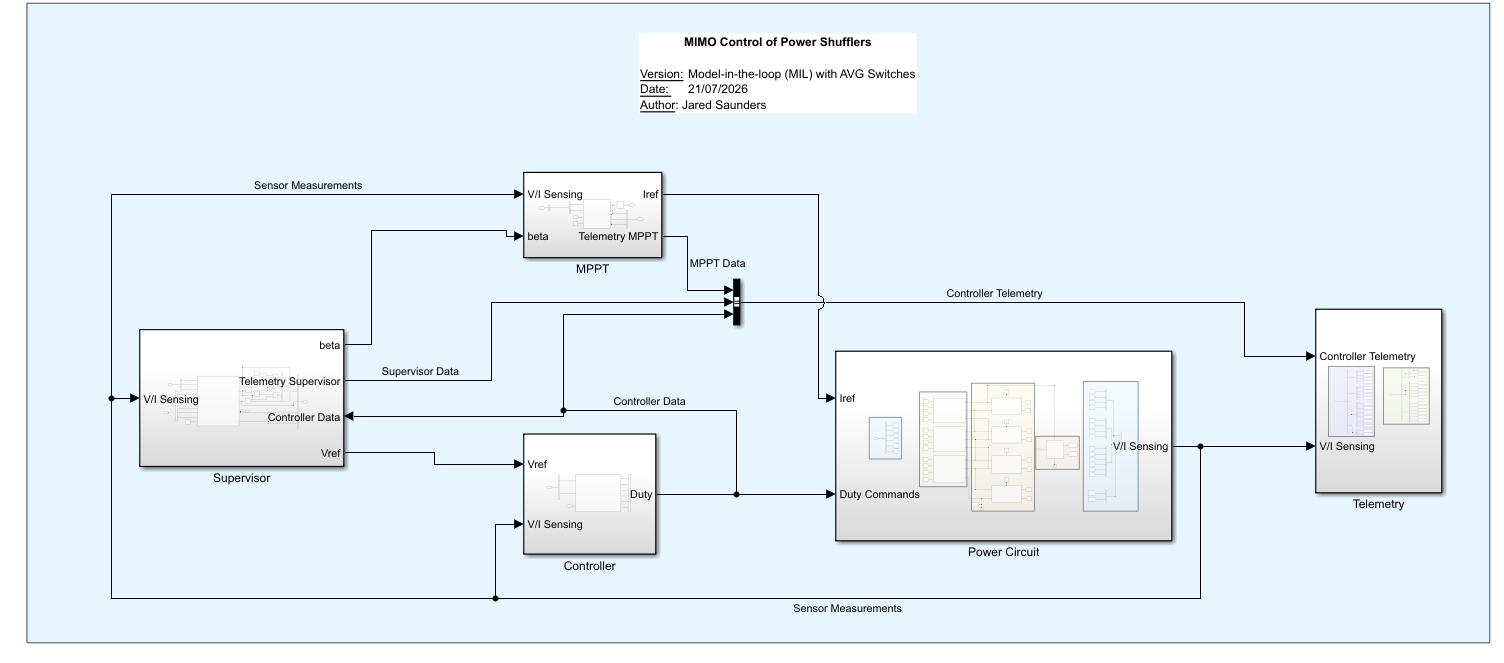
\includegraphics[width=0.92\linewidth]{img-013-015}
  \caption[{Simulink MIL model, top level}]{Simulink MIL model (\code{4\_Simulink/1\_MIL\_Model\_In\_The\_Loop}), top level: controller, supervisor, MPPT, power circuit and telemetry. The plant and the controller, supervisor and MPPT blocks are in \cref{fig:mil_plant,fig:mil_blocks}.}
  \label{fig:mil}
\end{figure}

Validation used a seven-test suite (\cref{tab:validate}): uniform irradiance, decoupling, half shade, shade with references, deep shade, MPPT under uniform irradiance and MPPT under shade. The pass criteria were $|\vd - r_v| < 0.25\V$ and $|\ic| < 1\A$ when tracking, an MPPT power of at least 98.5\,\% of the ceiling, and $|i_{diff}| \le 10\A$ in protection. All seven tests passed (\cref{tab:validate}; two are shown in \cref{fig:mil_validate}).

Software-in-the-loop (SIL) is an extension of MIL: the MATLAB Function blocks are replaced by C Caller blocks running the firmware's control core (\code{6\_RTOS/ctrl\_core}), and a bit-identical run against the MATLAB version, the golden replay, is the acceptance test. SIL is the cornerstone of the gain refinement pipeline, because the C that passes here is the C that the QSPICE DLL and the firmware compile.

\subsection{Component Selection}
\label{sec:components}
\Cref{fig:sysarch} shows the controller's data flow. The user reaches the system through the Raspberry Pi: over SSH and a parameter web page, with an IR remote, and through Grafana dashboards backed by InfluxDB, while an RGB LED and an LCD screen show the system state. The Pi flashes the Nucleo, exchanges commands and telemetry with it over UART, and reads the electronic load over USB. The Nucleo closes the loop on its own: it drives the eight PWM outputs, reads the current sensors on its ADCs and the voltage sensors over SPI, and the Pi never sits inside the control loop.

\begin{figure}[htbp]
  \centering
  % System architecture and data flow (after the presentation's controller data-flow diagram).
% Print size.
\begin{tikzpicture}[x=1cm,y=1cm,font=\sffamily\footnotesize,
    bx/.style={draw,rounded corners=3pt,minimum width=20mm,minimum height=7.5mm,align=center,thick},
    usr/.style={bx,draw=blue!55!black,fill=blue!8},
    pi/.style={bx,draw=green!45!black,fill=green!8},
    db/.style={bx,draw=orange!70!black,fill=orange!10},
    mcu/.style={bx,draw=violet!60!black,fill=violet!8},
    pl/.style={bx,draw=red!60!black,fill=red!8},
    ld/.style={bx,draw=gray!60!black,fill=gray!8},
    fl/.style={-{Stealth[length=1.8mm]},semithick},
    bl/.style={{Stealth[length=1.8mm]}-{Stealth[length=1.8mm]},semithick},
    l/.style={font=\sffamily\scriptsize,fill=white,inner sep=1pt}]
  % main row
  \node[usr] (user)  at (0,1.2)    {User};
  \node[pi]  (pi)    at (4.9,1.2)  {Raspberry Pi 4B};
  \node[mcu] (mcu)   at (9.8,1.2) {NUCLEO-G474RE};
  \node[pl]  (plant) at (14.25,1.2) {Shuffler PCB\\+ 3 PV modules};
  % Pi peripherals
  \node[pi]  (ir)    at (2.45,2.75) {IR receiver};
  \node[pi]  (led)   at (2.45,-0.35) {RGB LED};
  \node[pi]  (lcd)   at (2.45,-1.55) {LCD screen};
  % data services (Docker on the Pi)
  \node[db]  (graf)  at (0,4.3)   {Grafana};
  \node[db]  (infl)  at (4.9,4.3) {InfluxDB};
  % sensing
  \node[mcu] (cs)    at (12.0,-0.35) {TMCS1126 $\times$4};
  \node[mcu] (vs)    at (12.0,-1.55) {INA239 $\times$3};
  % electronic load
  \node[ld]  (el)    at (9.8,3.15) {Rigol DL3021\\e-load (CV)};
  % user interaction
  \draw[fl] (user) -- node[l,above]{SSH, params} (pi);
  \draw[fl] (user.north east) to[out=70,in=180] node[l,pos=0.3,left]{IR remote} (ir.west);
  \draw[fl] (ir.east) to[out=0,in=110] node[l,pos=0.5,above right]{button} ([xshift=-4mm]pi.north);
  \draw[fl] ([xshift=-4mm]pi.south) to[out=-100,in=0] node[l,pos=0.5,right]{colour = state} (led.east);
  \draw[fl] ([xshift=2mm]pi.south) to[out=-80,in=0] node[l,pos=0.5,right]{menu / telemetry} (lcd.east);
  \draw[fl] (led.west) to[out=180,in=-60] (user.south east);
  \draw[fl] (lcd.west) to[out=180,in=-90] node[l,pos=0.55,below left]{system state} (user.south);
  % logging
  \draw[fl] (pi) -- node[l,right,pos=0.72]{store telemetry} (infl);
  \draw[fl] (infl) -- node[l,above]{query} (graf);
  \draw[fl] (graf) -- node[l,left]{dashboards} (user);
  % control path
  \draw[fl] ([yshift=1.5mm]pi.east) -- node[l,above]{flash, commands} ([yshift=1.5mm]mcu.west);
  \draw[fl] ([yshift=-1.5mm]mcu.west) -- node[l,below]{telemetry 50 Hz} ([yshift=-1.5mm]pi.east);
  \draw[fl] (mcu) -- node[l,above]{PWM $\times$8} (plant);
  \draw[fl] ([xshift=4mm]plant.south) |- (cs.east);
  \draw[fl] ([xshift=4mm]plant.south) |- (vs.east);
  \draw[fl] (cs.west) -| node[l,pos=0.3,above]{ADC} ([xshift=-3mm]mcu.south);
  \draw[fl] (vs.west) -| node[l,pos=0.2,above]{SPI} ([xshift=3mm]mcu.south);
  % e-load
  \draw[bl] (el.east) -| node[l,pos=0.75,right]{string} (plant.north);
  \draw[bl] ([xshift=-2mm]pi.north east) |- node[l,pos=0.75,above]{USB-TMC (SCPI), 5 Hz} (el.west);
\end{tikzpicture}

  \caption[{Controller data flow}]{Controller data flow (after the presentation's data-flow diagram): the Raspberry Pi is the user interface, logger and flasher; the Nucleo closes the loop on its own.}
  \label{fig:sysarch}
\end{figure}

\Cref{fig:components} and \cref{tab:components} summarise the four controller components, with every figure taken from the manufacturers' datasheets. The STM32G474RE on the NUCLEO-G474RE board was chosen for its 170\,MHz clock, its five 12-bit ADCs and its high-resolution timer (HRTIM, 184\,ps resolution, with hardware dead time and complementary outputs) \cite{stm32g474_rm,mb1367_schematic}, together with its many general timers and its price; the ADC and PWM capability were the driving factors, and STM32CubeMX was used to allocate the peripherals (\cref{tab:periph_full}). The TMCS1126 Hall-effect sensor is galvanically isolated, so it can safely sit in series with the windings; the B4 variant gives 100\,mV/A about a 1.65\,V reference, a $\pm15.5$\,A linear range on a 3.3\,V supply and a 500\,kHz signal bandwidth \cite{tmcs1126_ds}. The INA239 was chosen because the higher-resolution INA229 was out of stock; it measures bus voltages up to 85\,V with a 16-bit ADC and 3.125\,mV resolution over SPI \cite{ina239_ds}. The three devices share SPI3 with separate chip selects, and their shunt inputs are tied off, so only the bus voltage and die temperature are used. The Raspberry Pi 4B \cite{rpi4_datasheet} was the safest way to add telemetry, remote control, a state display, connectivity and 5\,V / 3.3\,V distribution without adding complexity to the PCB; it hosts the web services and flashes the Nucleo, so the laptop never plugs into the system.

\begin{figure}[htbp]
  \centering
  \begin{subfigure}[b]{0.27\linewidth}\centering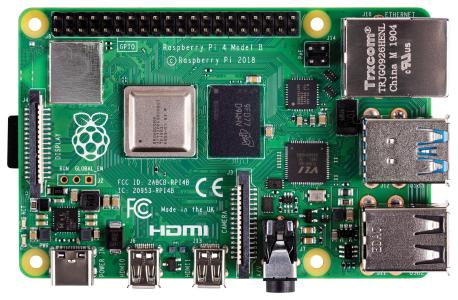
\includegraphics[height=3.0cm,keepaspectratio]{img-018-029}\caption{Raspberry Pi 4B \cite{rpi4_datasheet}}\end{subfigure}\hfill
  \begin{subfigure}[b]{0.20\linewidth}\centering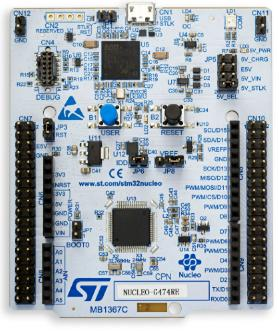
\includegraphics[height=3.0cm,keepaspectratio]{img-006-009}\caption{NUCLEO-G474RE \cite{mb1367_schematic}}\end{subfigure}\hfill
  \begin{subfigure}[b]{0.24\linewidth}\centering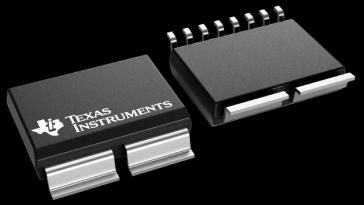
\includegraphics[width=\linewidth]{img-018-030}\caption{TMCS1126 \cite{tmcs1126_ds}}\end{subfigure}\hfill
  \begin{subfigure}[b]{0.24\linewidth}\centering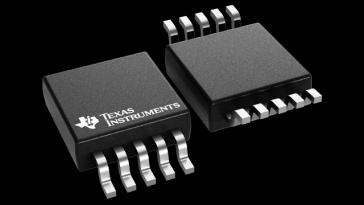
\includegraphics[width=\linewidth]{img-018-032}\caption{INA239 \cite{ina239_ds}}\end{subfigure}
  \caption[{Controller components}]{The controller components: microcomputer, microcontroller, Hall-effect current sensor and power monitor.}
  \label{fig:components}
\end{figure}

\begin{table}[htbp]\centering\small
\caption{Controller components and the datasheet figures behind their selection.}
\label{tab:components}
\begin{tabularx}{\linewidth}{l l X l}
\toprule
Role & Part & Key datasheet figures & Source\\
\midrule
Microcontroller & STM32G474RE (NUCLEO-G474RE) & Cortex-M4 at 170\,MHz; HRTIM with 184\,ps resolution, hardware dead time; five 12-bit ADCs & \cite{stm32g474_rm,mb1367_schematic}\\
Current sensor $\times$4 & TMCS1126B4AQDVGRQ1 & 100\,mV/A; $\pm15.5$\,A linear at 3.3\,V; 500\,kHz bandwidth; reinforced isolation, 5\,kV$_{\mathrm{RMS}}$ & \cite{tmcs1126_ds}\\
Voltage sensor $\times$3 & INA239AQDGSRQ1 & 0--85\,V bus input; 16-bit $\Delta\Sigma$ ADC, 3.125\,mV LSB; 10\,MHz SPI & \cite{ina239_ds}\\
Microcomputer & Raspberry Pi 4B & quad-core Cortex-A72 at 1.5\,GHz; Gigabit Ethernet, 802.11ac; 5\,V, 3\,A USB-C supply & \cite{rpi4_datasheet}\\
\bottomrule
\end{tabularx}
\end{table}

On the board (\cref{fig:routing}, \cref{app:firmware}) the ADC traces take the most direct path and are routed on the bottom layer to stay away from the switching nodes, the SPI forms a bus up and down the board, and the PWM and chip-select traces went wherever was convenient. One limitation of the Version 0 board was known before testing: the top INA239 (U10, chip select 3) sits behind an ISO7762 digital isolator that was wired backwards, so it cannot be read. The top module voltage is therefore reconstructed from the electronic load's readback, $V_{M1} = V_{str} - V_{M2} - V_{M3}$, which the Pi forwards to the Nucleo at 2\,Hz.

\subsection{Gain Refinement Pipeline}
\label{sec:gainpipe}
The gains are not tuned by hand. Each gain set starts with an identification, in which every input is stepped on a plant and the $4\times4$ DC gain matrix $G$ is measured (\cref{fig:gainpipe}). The design step turns $G$ into $M = G^{-1}\mathrm{diag}(k_I)$ and stores it, with the proportional ratios, the filter cut-off, the duty limits and a version string, in \code{shuffler\_params.json}. The generator \code{gen\_params.py} then writes \code{params.h}, which is compiled together with the same control core into all three harnesses. The version string travels in the telemetry, so every logged sample records which gain set produced it.

\begin{figure}[htbp]
  \centering
  % Gain refinement pipeline: identify G -> JSON gain set -> params.h + the one C core -> three harnesses.
% Print size.
\begin{tikzpicture}[x=1cm,y=1cm,font=\sffamily\footnotesize,
    b/.style={draw,rounded corners=2pt,thick,minimum width=31mm,minimum height=11mm,align=center,inner sep=3pt},
    f/.style={-{Stealth[length=1.8mm]},semithick},
    l/.style={font=\sffamily\scriptsize,fill=white,inner sep=1pt,align=center},
    hd/.style={font=\sffamily\scriptsize\bfseries,text=gray!40!black}]
  % column headings
  \node[hd] at (1.75,2.55) {1 identify};
  \node[hd] at (5.6,2.55) {2 design};
  \node[hd] at (10.0,2.55) {3 generate};
  \node[hd] at (14.0,2.55) {4 run the same code};
  % 1 identification plants
  \node[b,fill=blue!6]   (sim) at (1.75,1.3)  {Simulink carpark twin\\{\scriptsize step each $u$, measure $G$}};
  \node[b,fill=blue!6]   (qsp) at (1.75,-0.5) {QSPICE switching model\\{\scriptsize $u_d$ sweeps, $R_{sw}(\fsw)$}};
  % 2 gain set
  \node[b,fill=yellow!15,minimum height=29mm,minimum width=29mm] (json) at (5.6,0.4) {{\scriptsize\code{shuffler\_params.json}}\\[3pt]{\scriptsize $M = G^{-1}\mathrm{diag}(k_I)$}\\{\scriptsize $k_p$ ratios, $f_c$, duty limits}\\{\scriptsize version string}};
  % 3 generated header + shared core
  \node[b,fill=yellow!15] (ph)   at (10.0,1.3)  {{\scriptsize\code{params.h}}\\{\scriptsize $M$, $M_p$, $M^{-1}$ (float32)}};
  \node[b,fill=gray!8]    (core) at (10.0,-0.5) {{\scriptsize\code{ctrl\_core/*.c}}\\{\scriptsize C99, float32, no I/O}};
  \node[draw,densely dashed,rounded corners=4pt,gray,fit=(ph)(core),inner sep=4pt] (grp) {};
  % 4 harnesses
  \node[b,fill=green!8]  (sil) at (14.0,1.6)  {Simulink SIL\\{\scriptsize C Caller blocks}};
  \node[b,fill=green!8]  (dll) at (14.0,0.4)  {QSPICE DLL\\{\scriptsize the ``Nucleo'' block}};
  \node[b,fill=orange!10] (fw) at (14.0,-0.8) {firmware ISR\\{\scriptsize\code{stack\_step()}, 10 kHz}};
  % flow
  \draw[f] (sim.east) -- (json.west |- sim.east);
  \draw[f] (qsp.east) -- (json.west |- qsp.east);
  \draw[f] (json.east |- ph.west) -- (ph.west);
  \node[font=\scriptsize,align=center,anchor=north] at ($(json.east |- ph.west)!0.5!(ph.west)+(0,-0.12)$) {\code{gen\_}\\\code{params}\\\code{.py}};
  \foreach \t in {sil,dll,fw}{\draw[f] (grp.east |- \t.west) -- (\t.west);}
  % run-time knob
  \node[font=\sffamily\scriptsize,align=center,text=gray!30!black] at (8.1,-1.95)
       {run time: $u = k\,(M_p e + M\xi)$ with one gain scale $k$ (\code{kscale}, boot value 0.3); a staged gain set is applied bumplessly ($\xi = M^{-1}u_{act}$)};
\end{tikzpicture}

  \caption[{Gain refinement pipeline}]{Gain refinement pipeline: identification in Simulink or QSPICE, one JSON gain set, a generated \code{params.h}, and the same C core in the Simulink SIL harness, the QSPICE DLL and the firmware.}
  \label{fig:gainpipe}
\end{figure}

Two identification plants were used. The Simulink carpark twin (\cref{fig:twin}, \cref{app:simfigs}) was updated to match the experiments: power sources for the NGE103 channels or the KAUSSP80 cells, the DL3021 in constant-voltage mode, a plant reduced to three modules, and a sensing block that reproduces the INA round robin (1\,kHz, 3.125\,mV resolution), the 12-bit hall ADC, optional noise (2\,mV and 20\,mA rms) and the Pi's 2\,Hz $V_{M1}$ path. The control architecture was also integrated into the hardware teammate's QSPICE model (\cref{fig:qspice}): a controller component wraps the unchanged C core as a DLL, sampling at 10\,kHz with the INA values held at 1\,kHz and the hall readings quantised, and drives HRTIM-style comparators. The sensors are modelled too, including the TMCS1126's 500\,kHz pole and the reversed B-phase sensors.
The two plants agree on the voltage block of $G$ ($\vd/\uc \approx -46\V$ per unit on both) but not on the current block: 742 against 142\,A per unit at 200\,kHz (\cref{tab:G}). The difference is an effective resistance in the switching plant. During each dead time the switch-node capacitance must be commutated, which costs volt-seconds in proportion to the current and appears as
\begin{equation}
  R_{sw} = 64\,C_p\,\fsw^3\,(L+M)^2,
\end{equation}
0.29, 0.80 and 1.70\,$\Omega$ at 200, 300 and 400\,kHz (\cref{app:rsw}). The Simulink bench gain set was therefore rejected for hardware: QSPICE is the arbiter and Simulink the source. A new switching frequency needs a new identification and gain set (\cref{app:gains}). The switching frequency is a parameter in QSPICE and a compile-time define (\code{HW\_PWM\_KHZ}) in the firmware, and \code{run\_scenarios.m} and \code{run\_scenarios.py} run every setup and gain scale.

\subsection{Firmware / Software}
\label{sec:firmware}
The firmware is a bare-metal C application on the STM32G474, built with the STM32CubeMX HAL, CMake, Ninja and the \code{arm-none-eabi} toolchain at \code{-O2}. It contains the portable control core (\code{ctrl\_core}: controller, supervisor, MPPT, reconstruction and the stack that schedules them), drivers for the HRTIM, ADC, SPI and UART, a supervisory state machine and a line-based telemetry and command protocol (\cref{app:firmware}). FreeRTOS was planned, but the shipped firmware is a superloop with interrupts: the time-critical work runs in interrupts with fixed priorities, and the slower tasks run from the main loop on millisecond ticks. Moving to a real-time operating system is left as future work (\cref{sec:conclusion}).

In order of priority, the firmware runs the E-stop interrupt, the 10\,kHz control interrupt triggered by the HRTIM master timer, INA polling at 1\,kHz, the safety checks and state machine at 100\,Hz, telemetry at 50\,Hz and command parsing. The safety path (the over-current latch inside the control interrupt, the E-stop interrupt and the 0.3\,s independent watchdog) never depends on the main loop. The peripheral settings are in \cref{tab:periph_full}. The hall currents are sampled by four HRTIM-triggered ADC conversions per switching period and box-averaged over the whole control tick (\cref{fig:adc}, \cref{app:firmware}); the average acts as a comb filter with nulls at $\fsw$ and its harmonics, so the controller sees the average winding current free of switching ripple.

\begin{figure}[htbp]
  \centering
  % Deployed control architecture (10 kHz ISR forward path, feedback, 1 kHz supervisor).  Print size.
\begin{tikzpicture}[x=1cm,y=1cm,font=\sffamily\footnotesize,
    b/.style={draw,rounded corners=2pt,thick,minimum height=10mm,align=center,inner sep=3pt},
    f/.style={-{Stealth[length=1.8mm]},semithick},
    l/.style={font=\sffamily\scriptsize,fill=white,inner sep=1pt}]
  % forward path
  \node[b,fill=blue!6,minimum width=22mm]  (ref)  at (1.1,0)  {references\\$r = [V_{ref}+r_v,\,0]$};
  \node[draw,circle,thick,inner sep=1.5pt] (sum)  at (3.15,0)  {$\Sigma$};
  \node[b,fill=blue!6,minimum width=25mm]  (pi)   at (5.55,0)  {MIMO PI, 10 kHz\\$u = k\,(M_p e + M\xi)$};
  \node[b,fill=blue!6,minimum width=19mm]  (map)  at (9.05,0)   {duty map\\+ limits};
  \node[b,fill=orange!10,minimum width=19mm] (pwm) at (11.95,0) {HRTIM PWM\\4 legs};
  \node[b,fill=yellow!15,minimum width=17mm] (pl)  at (14.85,0) {2 shufflers\\3 modules};
  % feedback path
  \node[b,fill=green!8,minimum width=27mm]  (sen)  at (13.3,-2.1) {TMCS1126 $\times$4 $\rightarrow$ ADC\\INA239 $\times$3 $\rightarrow$ SPI};
  \node[b,fill=green!8,minimum width=27mm]  (lpf)  at (6.8,-2.1)  {reconstruction\\+ LPF $f_c = 2$ kHz};
  % supervisor
  \node[b,fill=red!8,minimum width=27mm]   (sup)  at (5.55,-3.7)  {supervisor, 1 kHz\\stress $\rightarrow\beta\rightarrow r_v$};
  % wiring
  \draw[f] (ref) -- (sum);
  \draw[f] (sum) -- node[l,above]{$e$} (pi);
  \draw[f] (pi) -- node[l,above]{$u_c, u_d$} (map);
  \draw[f] (map) -- node[l,above]{$d_A, d_B$} (pwm);
  \draw[f] (pwm) -- (pl);
  \draw[f] (pl.south) |- node[l,pos=0.25,right]{$V_M$, $I_L$} (sen.east);
  \draw[f] (sen) -- (lpf);
  \draw[f] (lpf.west) -| node[l,pos=0.2,above]{$y = [v_d,\ i_c]$} node[l,pos=0.93,left]{$-$} (sum.south);
  \draw[f] (sen.south) |- node[l,pos=0.75,below]{$I_L$, module currents} (sup.east);
  \draw[f] ([xshift=-3mm]map.south) |- node[l,pos=0.6,above]{applied duties} ([yshift=2mm]sup.east);
  \draw[f] (sup.west) -| node[l,pos=0.25,below]{$r_v$ (one-tick delay)} (ref.south);
\end{tikzpicture}

  \caption[{Deployed control architecture}]{Deployed control architecture: the 10\,kHz forward path, the measurement feedback, and the 1\,kHz supervisor that sets the voltage-difference references.}
  \label{fig:ctrlloop}
\end{figure}

Every 100\,$\mu$s the control interrupt reconstructs $\vd$ and $\ic$ from the sensors, filters them at 2\,kHz, runs the MIMO PI and maps $\uc$ and $\ud$ to the leg duties $d_A = \tfrac12(1+\uc+\ud)$ and $d_B = \tfrac12(1+\uc-\ud)$, with limits and a slew of 0.01 per tick (\cref{fig:ctrlloop}). Every millisecond the supervisor forms a stress index from the filtered differential currents and the duty excursion, integrates its governor gain $\beta$ and relaxes the voltage-difference references $r_v$, which reach the controller one tick later. The pseudocode for the interrupt, soft-start, supervisor and state machine is in \cref{app:pseudo}.

\begin{figure}[htbp]
  \centering
  % Firmware supervisory state machine (6_RTOS/App/app.c, 100 Hz task).  Print size.
\begin{tikzpicture}[x=1cm,y=1cm,font=\sffamily\footnotesize,
    s/.style={draw,ellipse,thick,draw=blue!50!black,fill=blue!6,minimum width=20mm,minimum height=10mm,align=center,inner sep=1pt},
    sf/.style={s,draw=red!60!black,fill=red!10},
    t/.style={-{Stealth[length=1.8mm]},semithick},
    l/.style={font=\sffamily\scriptsize,fill=white,inner sep=1pt,align=center}]
  \node[s] (boot) at (0.75,0)  {BOOT};
  \node[s] (self) at (3.65,0)  {SELFTEST\\[-1pt]{\scriptsize INA init, hall zero}};
  \node[s] (idle) at (7.15,0)  {IDLE\\[-1pt]{\scriptsize legs off, pre-bias $d_0$}};
  \node[s] (ss)   at (10.85,0) {SOFTSTART\\[-1pt]{\scriptsize 150 ms duty ramp}};
  \node[s] (run)  at (14.15,0) {RUN\\[-1pt]{\scriptsize OL / CL modes}};
  \node[s] (stop) at (10.85,-2.4) {STOP\\[-1pt]{\scriptsize legs off}};
  \node[sf] (flt) at (7.15,-3.9) {FAULT\\[-1pt]{\scriptsize outputs off, latched}};
  \draw[t] (boot) -- (self);
  \draw[t] (self) -- node[l,above]{ok} (idle);
  \draw[t] (idle) -- node[l,above=4mm]{\code{C,EN,1}\\mode $\neq$ IDLE} (ss);
  \draw[t] (ss) -- node[l,above=4mm]{ramp\\done} (run);
  \draw[t] (ss) -- node[l,right]{\code{C,EN,0}} (stop);
  \draw[t] (run) |- node[l,pos=0.25,right]{\code{C,EN,0} or\\mode IDLE} (stop);
  \draw[t] (stop) -| node[l,pos=0.3,below]{next tick} ([xshift=6mm]idle.south);
  \draw[t] (self) |- node[l,pos=0.3,left]{zero-cal or\\INA fail} (flt);
  \draw[t,red!60!black] (run.south) |- (flt.east);
  \node[l,text=red!60!black,anchor=north] at (11.4,-4.0) {\code{trip()} from any state: OC, OV/UV, E-stop,\\over-temperature, comms watchdog, main-loop stall};
  \draw[t] ([xshift=-4mm]flt.north) -- node[l,left]{\code{C,CLEAR}\\(E-stop released)} ([xshift=-4mm]idle.south);
\end{tikzpicture}

  \caption{Supervisory state machine of the firmware (\code{6\_RTOS/App/app.c}, 100\,Hz task).}
  \label{fig:fsm}
\end{figure}

The state machine (\cref{fig:fsm}) starts in BOOT and runs SELFTEST, which initialises the INA239s and zero-calibrates the hall sensors; a failure latches FAULT. From IDLE, an enable command (\code{C,EN,1}) with a non-idle mode starts SOFTSTART, which ramps the duties to their target over 150\,ms before entering RUN. Disabling or selecting IDLE passes through STOP, which turns the legs off, and returns to IDLE on the next tick. Any trip (over-current, over- or under-voltage, E-stop, over-temperature, the communications watchdog or a main-loop stall) switches the outputs off first and latches FAULT, and \code{C,CLEAR} returns to IDLE only once the E-stop is released.
On the Pi, Docker runs InfluxDB and Grafana, \code{pod.py} bridges the serial telemetry and drives the LCD, LED and IR receiver, and \code{eload.py} polls the DL3021 at 5\,Hz and forwards $V_{str}$ to the Nucleo at 2\,Hz (\cref{app:firmware}). The physical signals were checked on the oscilloscope: the dead time and the 180$^\circ$ interleave at 200, 300 and 400\,kHz, and the alignment of the ADC triggers (\cref{fig:scope}).

\subsubsection{Experimental setup and test plan}
\label{sec:setup}
The two set-ups are compared in \cref{tab:setup} and photographed in \cref{fig:setupphotos} (\cref{app:journey}). The tests answer five questions: (i) does the open loop behave as modelled ($V_{M2}/(V_{M2}+V_{M3}) = 1-d$, $\vd = -R_m\im$, a duty-step gain of $-\Vbar$); (ii) does the closed loop regulate ($\vd \rightarrow 0$, $\ic \rightarrow 0$, with the steady-state error and noise measured against $k$ and $\fsw$); (iii) does it reject disturbances (supply and load steps on the bench, shade in the sun); (iv) how much stability margin is there (raising $k$ until the loop misbehaves); and (v) how much energy is returned under shade (delivered against returned power).

\begin{table}[htbp]\centering\small
\caption{Bench and solar experimental set-ups.}
\label{tab:setup}
\begin{tabularx}{\linewidth}{l X X}
\toprule
 & Bench, 16 Oct 2026 (lab) & Solar, 20 Oct 2026 (carpark)\\
\midrule
Modules & R\&S NGE103 three-channel supply \cite{rohde_nge100_ds}, 25\,V set, current limits 0.8 / 1.0 / 1.3\,A & 3 $\times$ KickAss KAUSSP80 \cite{kaussp80_ds}: 80\,W, $V_{oc}$ 25.1\,V, $I_{sc}$ 4.35\,A, $V_{mp} \approx 20.5$\,V\\
Load & Rigol DL3021 \cite{rigol_dl3000_ds} in CV at 70\,V (steps 60--125\,V) & DL3021 in CV at 61\,V ($\approx 3V_{mp}$)\\
Mismatch & supply current limits & cardboard or a shirt over one module\\
Switching frequency & 200, 300, 400\,kHz, one gain set per $\fsw$ & 200\,kHz only\\
Gain scale & per run & sweep $k = 0.1$ to 0.8\\
Instruments & oscilloscope (dead time, interleave) & telemetry and e-load log only\\
Supply for Pi and laptop & mains & battery and inverter\\
Windows & 10 (B01--B09 and B01s, \cref{tab:T1}) & 11, peak sun 15:04--15:13, minimal sun after 15:48\\
\bottomrule
\end{tabularx}
\end{table}
The two set-ups test different things. The supply channels are stiff current limits with no I--V curve and no irradiance, so the bench exercises the loop and the gain set for each switching frequency. The sun exercises the plant the controller was designed for, but only at 200\,kHz and at the irradiance the day gave. The full test matrix is \cref{tab:T1} (21 windows); the pre-flight checklist and power-up order are in the repository (\code{0\_Documentation/experiment\_checklist.md}).

Every metric has one definition for every phase (\code{stepmetrics.py}, \cref{app:synth}).

The hardware cannot resolve the loop dynamics. Telemetry arrives at about 44\,Hz (11--14\,Hz on three 200\,kHz bench runs) while the loop time constants are 1--10\,ms, so hardware rise and settling times are bounds ($\le 23\ms$, one telemetry frame). The hardware does resolve steady-state error, noise, second-scale disturbances, duty-step amplitudes and energy, and the step response is taken from the models.

\subsection{Risks}
\label{sec:risks}
The risk register from the proposal (\cref{tab:risk}, \cref{app:risk}) was kept and updated through the project, and the earlier shuffler's failure (\cref{sec:lit_dpp}) is why protection was designed in from the start rather than added later. Several risks materialised. Scope creep compromised the PCB revisions and features, leaving a single board. Firmware faults were contained by the E-stop, fault latching and state telemetry: faults 0x10 (module under-voltage) and 0x2000 (main-loop stall) tripped three times on 16 Oct when gains were applied live (\cref{tab:T3kscale}), and each time the outputs switched off safely. The averaged model was inaccurate, over-estimating the current-loop gain fivefold, but this was caught in QSPICE before any hardware ran. The top voltage sensor (U10) could not be read and was replaced by the e-load readback. Electrical safety (component ratings and a 15\,A string fuse) and outdoor testing (sun, fire and rain) were managed by procedure, and no risk led to injury or to component damage (U10's isolator was wired backwards at assembly).

\subsection{Ethics}
\label{sec:ethics}
Electrical safety followed QUT's HSE protocols for electrical workspaces: PPE, a 15\,A string fuse, hardware and software E-stops, over-current, over- and under-voltage and over-temperature envelopes in the firmware, and a rule that the system was never left energised unattended. For data security and privacy, all services are hosted locally on the Raspberry Pi with authentication and no cloud connection, only sensed data and internal states are streamed, and credentials are excluded from version control. For integrity, AI assistance (Claude) was used for derivation checking, scripting and the results pipeline; every result can be reproduced from the repository (\code{make all}). 

\subsection{Sustainability}
\label{sec:sustainability}
The project was sustained by constant collaboration (bi-weekly team meetings, a shared GitHub repository and defined hand-over milestones with the hardware teammate). The future of the project is supported by every folder of the repository containing a README, videos recordings expaining the project and regenerable results are all in the repository. Because the shuffler processes only the mismatch power, its component ratings and losses scale with the shading rather than with the string power, which supports more efficient use of existing solar capacity (UN SDG~7.3).
